\subsection{Le dipôle court: $l \ll \lambda$}
Le gain de l'antenne dans le plan E est représenté dans la figure \ref{fig:gain21}.
\begin{figure}[htbp]
  \centering
  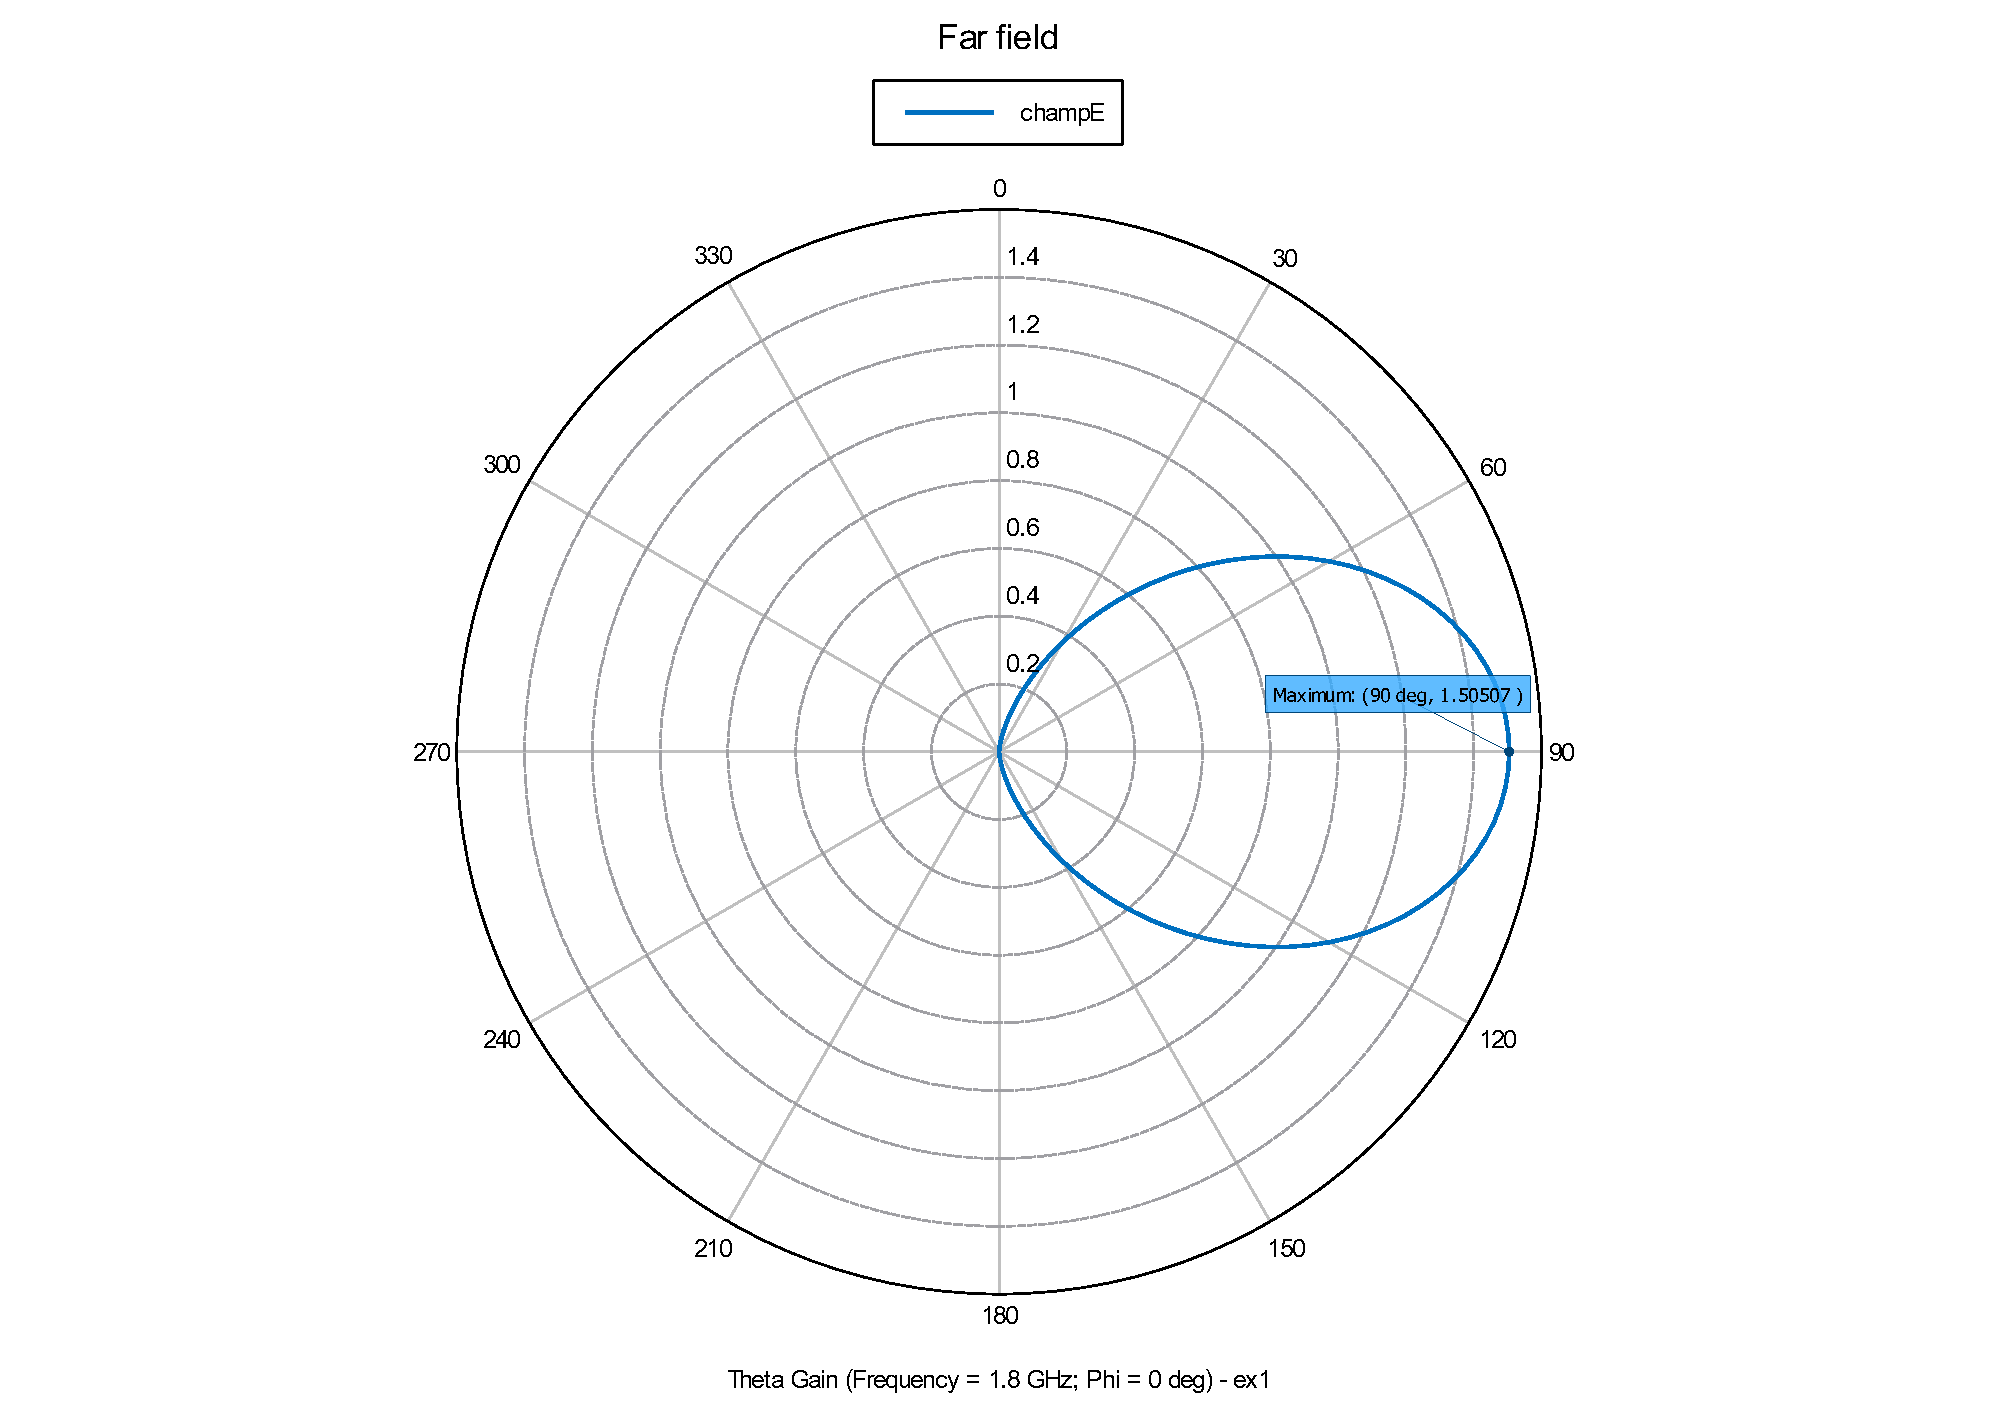
\includegraphics[width=\textwidth]{gain21.pdf}
  \caption{Diagramme de rayonnement du dipôle court dans le plan E.\label{fig:gain21}}
\end{figure}
Le gain n'est pas représenté pour $\SI{180}{\degree}<\theta<\SI{360}{\degree}$, ce qui n'est pas important puisque l'on sait que le problème présente une symétrie cylindrique. Pour la même raison, les diagrammes dans le plan H ne sont pas donnés ici, mais se déduisent logiquement de la figure \ref{fig:gain21}: le gain est indépendant de $\phi$. Sa composante $\theta$ vaut la gain maximal du diagramme de rayonnement dans le plan E, et sa composante $\phi$ vaut $0$.

Sur la figure \ref{fig:gain21}, on lit un gain maximal de $\num{1.51} = \SI{1.79}{\deci\bel}$, ce qui est légèrement supérieur à la valeur $\frac{3}{2} = \SI{1.76}{\deci\bel}$ prédite par l'approximation du dipôle de Hertz. Ceci est logique puisque la directivité maximale augmente lorsqu'on augmente la longueur du dipôle.

La résistance de rayonnement est représentée en fonction de la fréquence à la figure \ref{fig:Rar21}.
\begin{figure}[htbp]
  \centering
  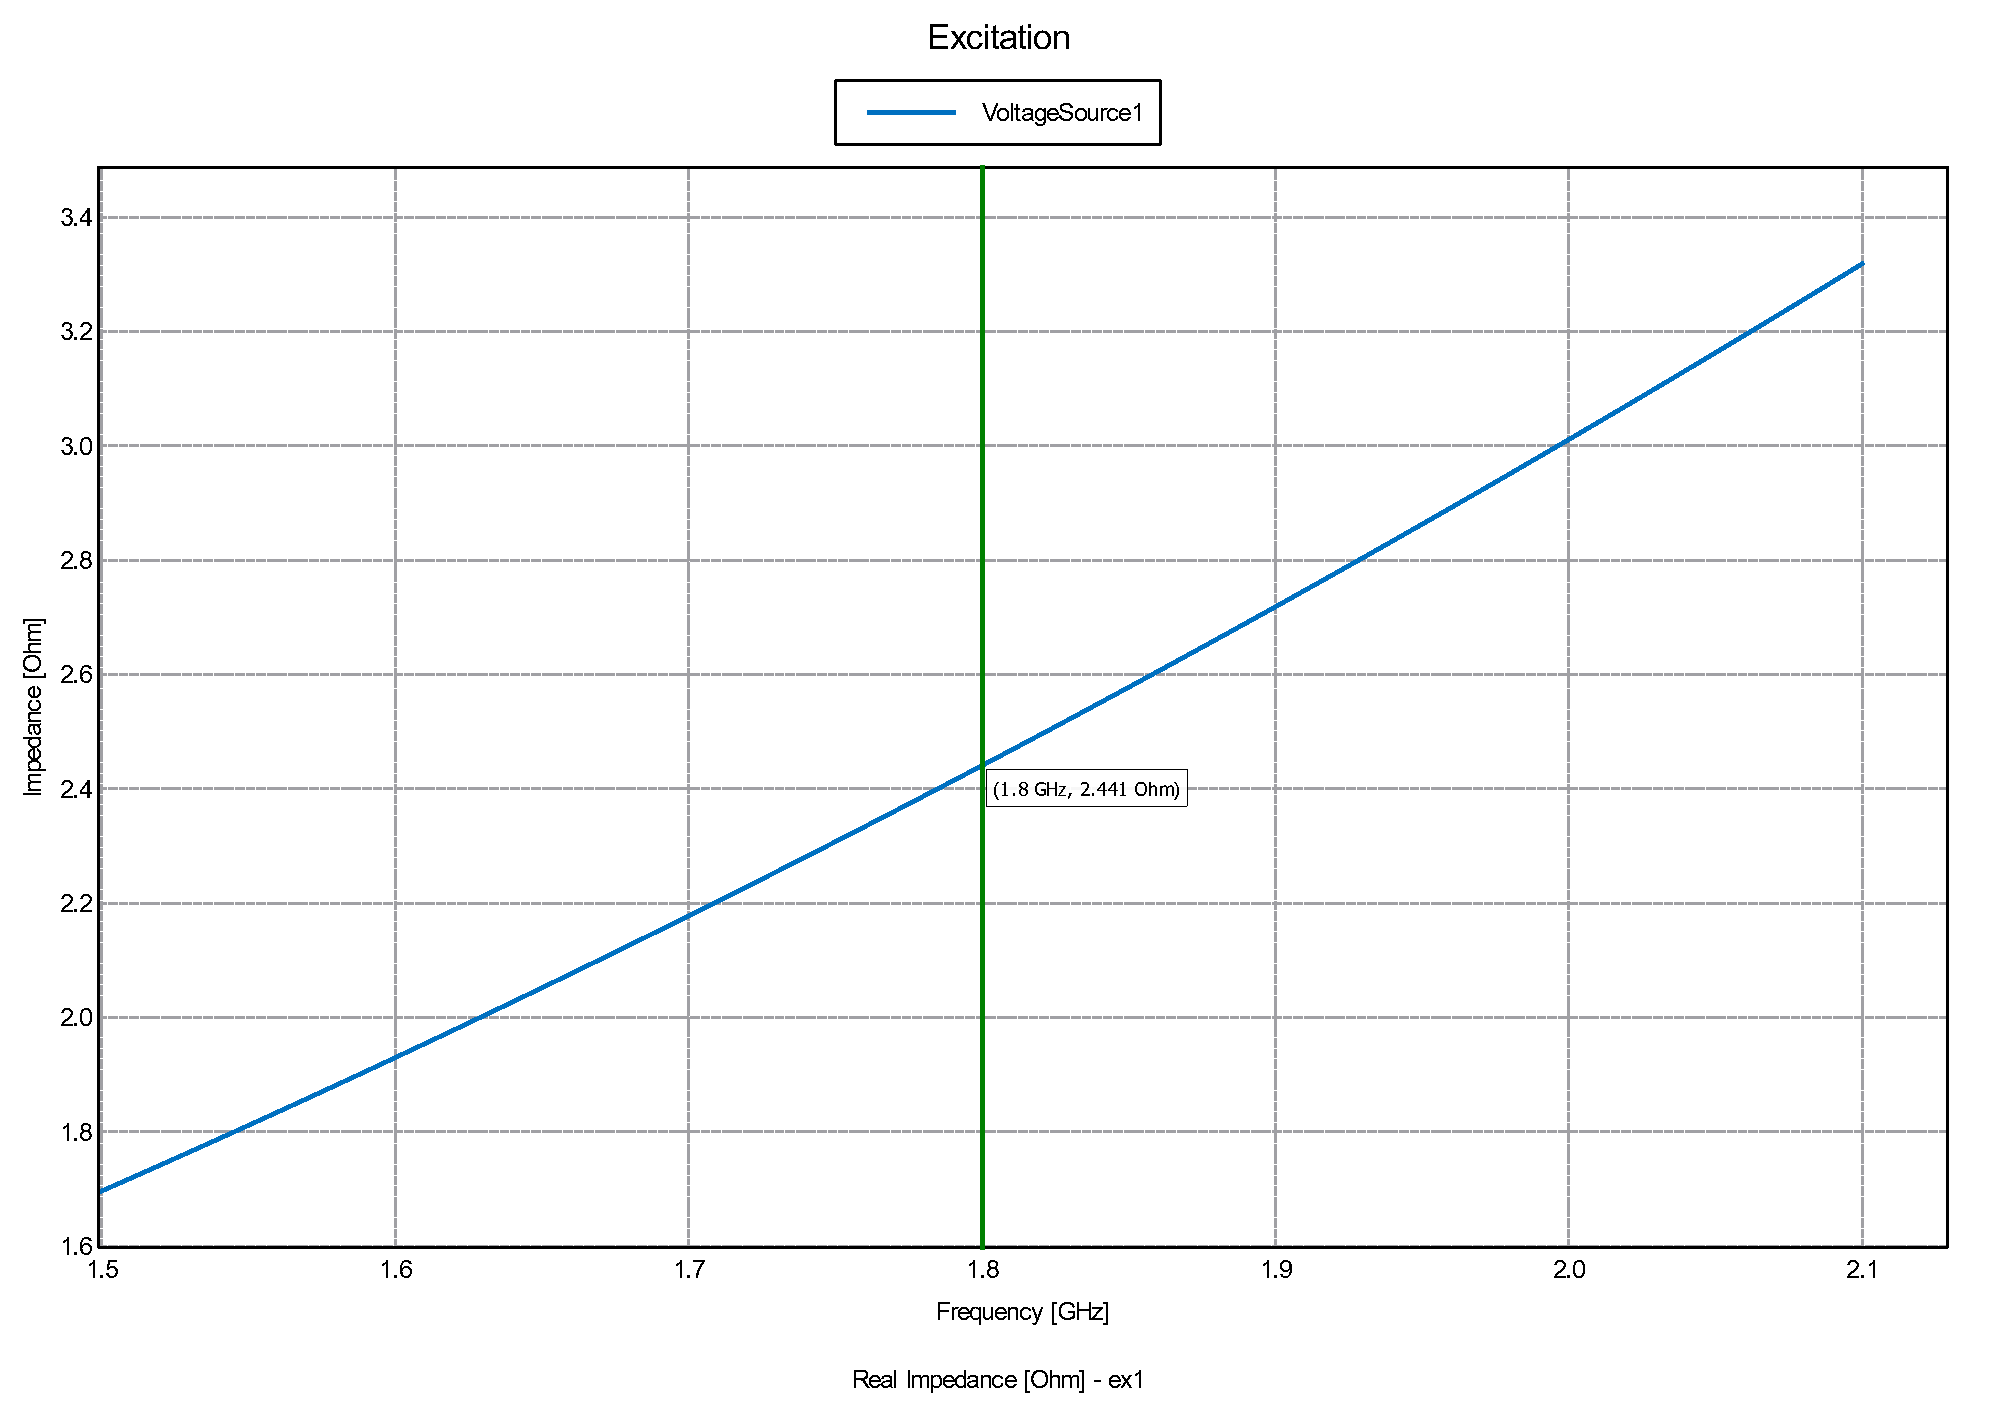
\includegraphics[width=\textwidth]{Rar21.pdf}
  \caption{Résistance de rayonnement du dipôle court en fonction de la fréquence.\label{fig:Rar21}}
\end{figure}
Puisque le fil est modélisé par un conducteur parfait et que les connections ne sont pas prises en compte, la résistance ohmique est considérée comme nulle. Sur la figure \ref{fig:Rar21}, on lit $R_{ar} = \SI{2.44}{\ohm}$ pour $f = \SI{1.8}{\giga\hertz}$, ce qui est très inférieur à la valeur $R_{ar} = 80 \left (\frac{\pi l}{\lambda} \right ) ^2 = \SI{7.90}{\ohm}$ prédite par l'approximation de l'élément de courant.

A partir de cette valeur, on obtient la fraction de puissance consommée par l'antenne en calculant d'abord $\Gamma_L$ puis en utilisant la relation \ref{eqn:puissance délivrée}.
\begin{align*}
\Gamma_L = \frac{Z_L - Z_c}{Z_L + Z_c} &= 0.91\numberthis\label{eqn:reflect}\\
\frac{P_L}{P_{in}} &= \SI{17.7}{\percent}
\end{align*}
L'adaptation d'impédance est donc très mauvaise. Ceci peut-être résolu en utilisant un dipôle demi-onde, comme nous le verrons dans la prochaine section.

\subsection{Le dipôle demi-onde: $l = \frac{\lambda}{2}$}
Le gain dans le plan E est représenté dans un diagramme polaire à la figure \ref{fig:gain22}.
\begin{figure}[htbp]
  \centering
  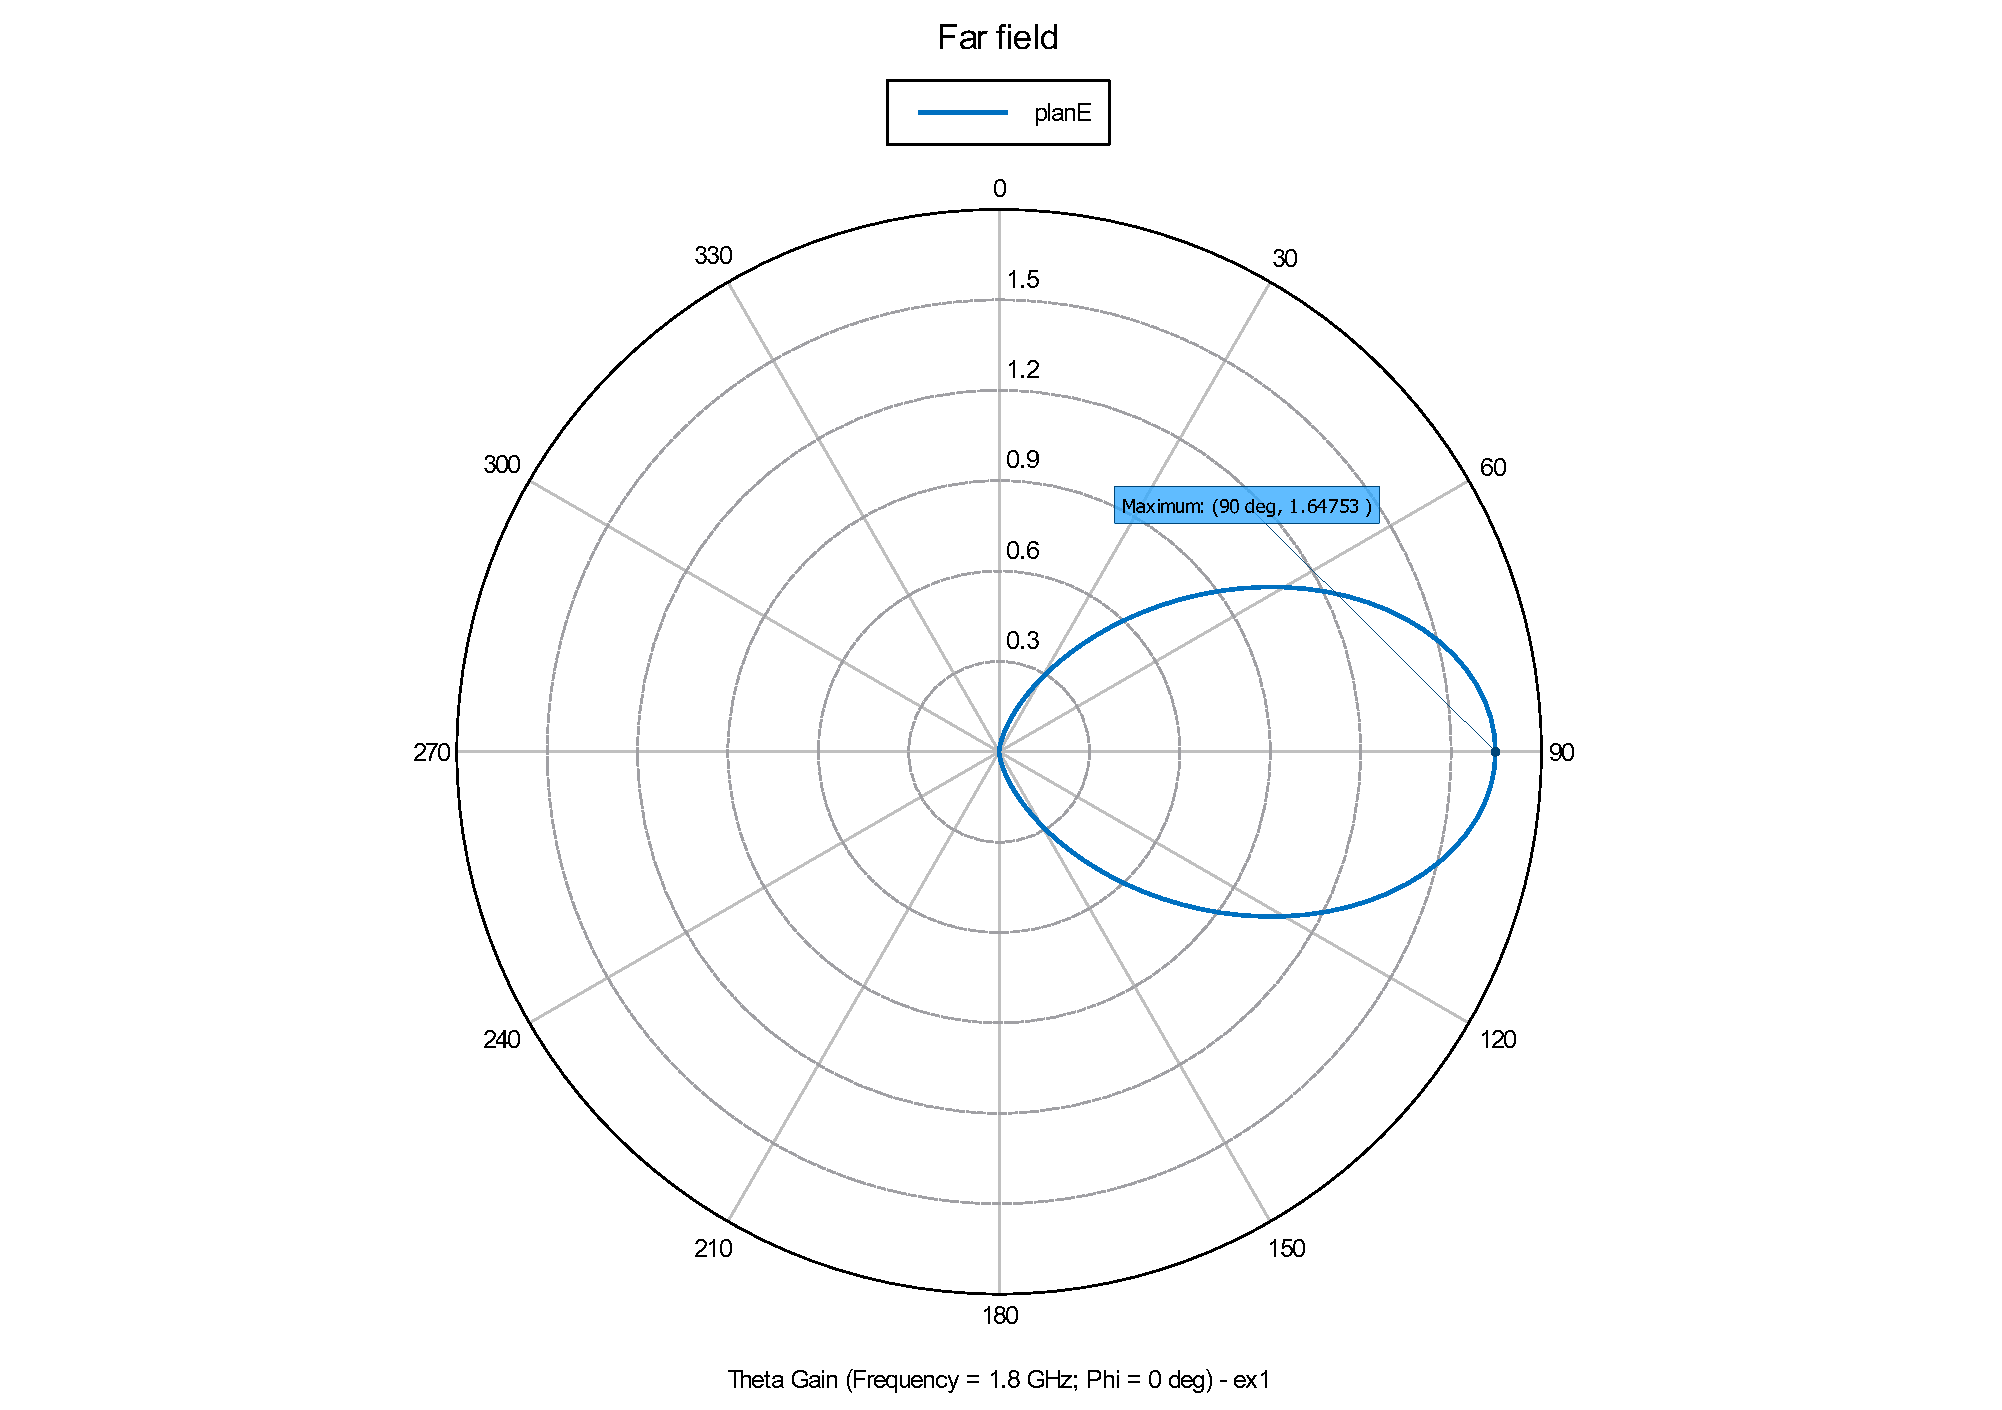
\includegraphics[width = \textwidth]{Rar22.pdf}
  \caption{Diagramme de rayonnement du dipôle demi-onde dans le plan E.\label{fig:gain22}}
\end{figure}
Les propriétés de symétrie de la figure \ref{fig:gain21} s'appliquent toujours. On lit sur le diagramme de rayonnement un gain maximal de \num{1.65}, ce qui est légèrement inférieur à la valeur de \num{1.7} prédite avec l'approximation $\left ( \frac{\cos(\frac{\pi}{2}\cos\theta)}{\sin\theta} \right ) ^2 \simeq \sin^3 \theta$.

Sur la figure \ref{fig:Z22},
\begin{figure}[htbp]
  \centering
  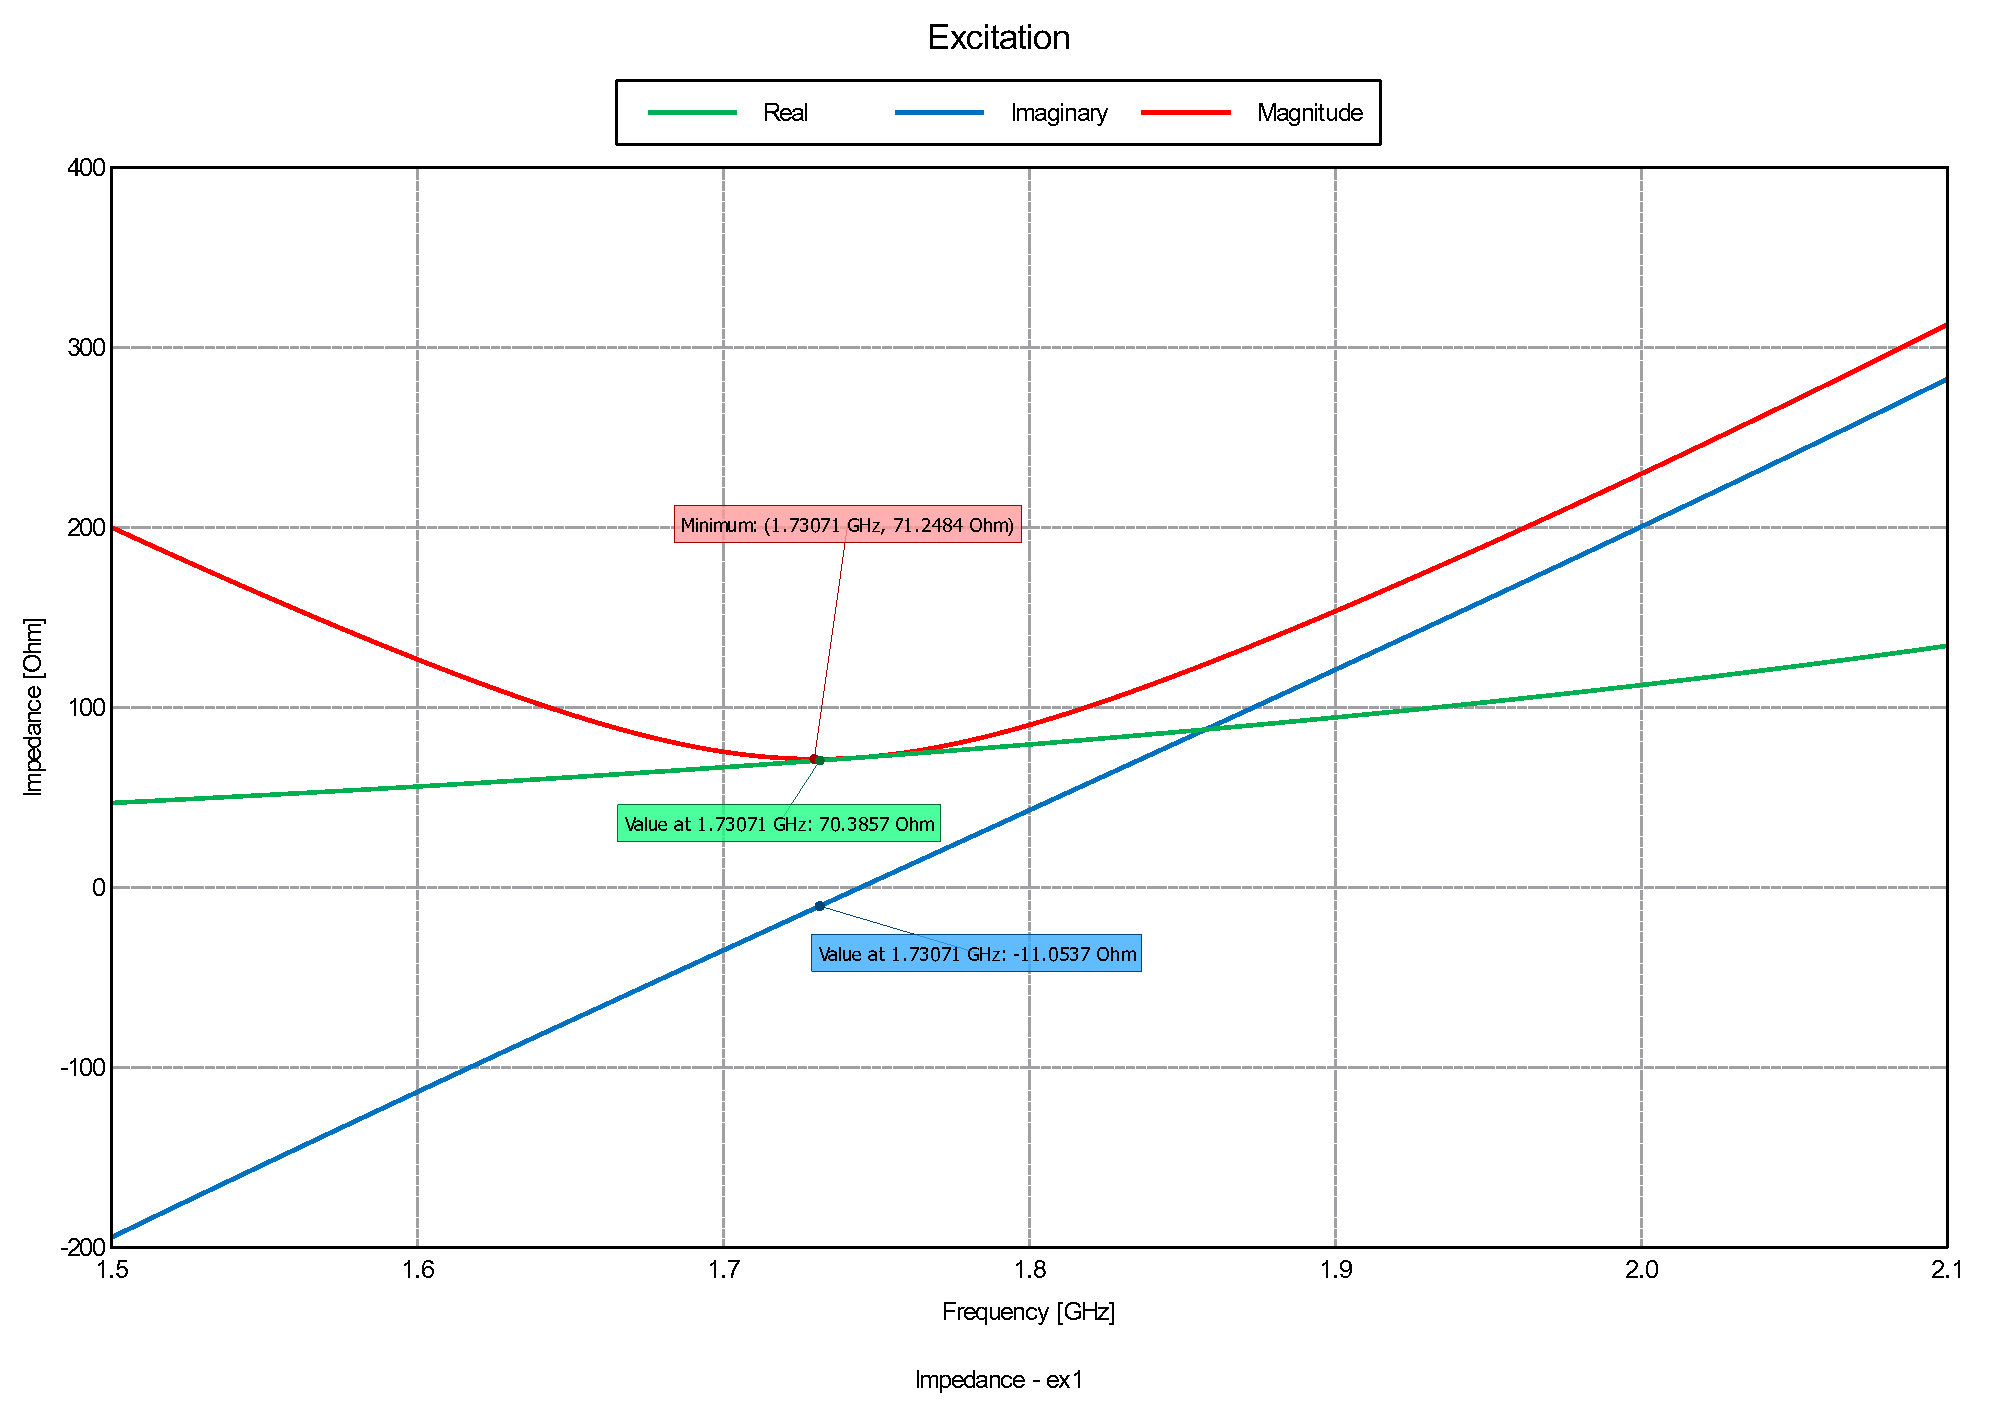
\includegraphics[width = \textwidth]{Z22.pdf}
  \caption{Parties réelle et imaginaire et module de l'impédance de l'antenne en fonction de la fréquence.\label{fig:Z22}}
\end{figure}
on constate que la partie imaginaire de l'impédance croît linéairement avec la fréquence, et ce beaucoup plus rapidement que la partie réelle qui peut est considérée comme quasi constante. De plus, comme la partie imaginaire évolue d'une valeur négative vers une valeur positive, le module de l'impédance n'est lui pas monotone et présente un minimum qui est approximativement donné par le zéro de la partie imaginaire. Sur la figure \ref{fig:Z22}, ce point se situe à \SI{1.73}{\giga\hertz}. Nous allons maintenant essayer de le déplacer à \SI{1.8}{\giga\hertz} en modifiant la longueur du dipôle.

Ceci est fait à la figure \ref{fig:Z022}.
\begin{figure}[htbp]
  \centering
  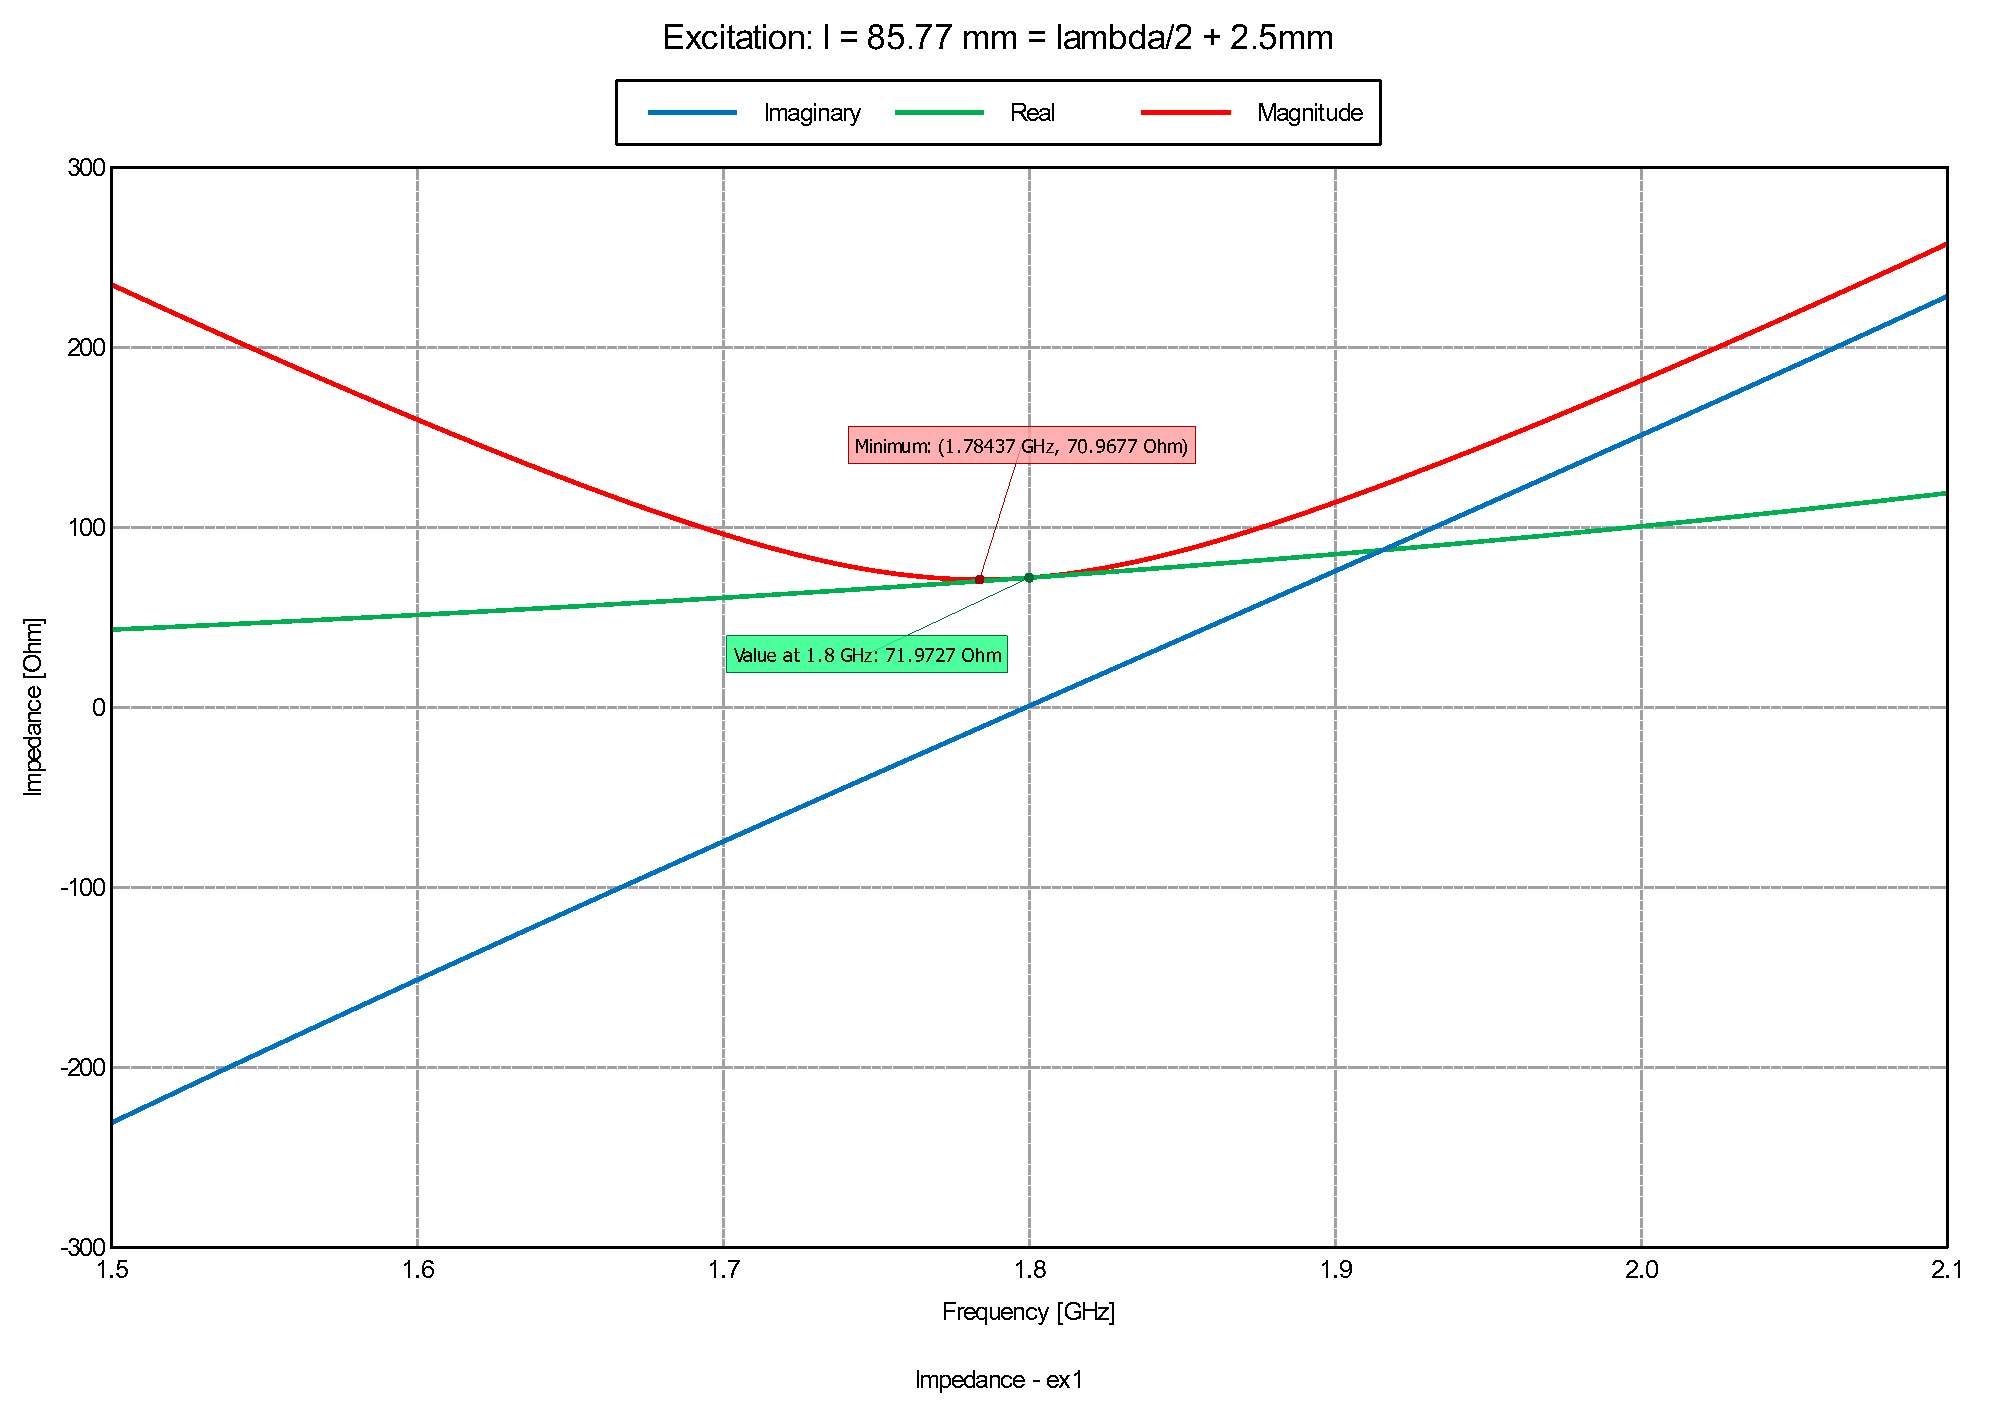
\includegraphics[width = \textwidth]{Z022.pdf}
  \caption{Parties réelle et imaginaire et module de l'impédance de l'antenne adaptée pour \SI{1.8}{\giga\hertz} en fonction de la fréquence.\label{fig:Z022}}
\end{figure}
La partie imaginaire de l'impédance s'annule bien en $f = \SI{1.8}{\giga\hertz}$ et le module de l'impédance de rayonnement est donc proche de son minimum.

En utilisant la relation \ref{eqn:reflect}, on obtient $\Gamma_L = 0.027 = \SI{-31.2}{\deci\bel}$ pour $Z_c = \SI{75}{\ohm}$. Ceci est confirmé par la simulation, comme le montre la figure \ref{fig:gamma22}.
\begin{figure}[htbp]
  \centering
  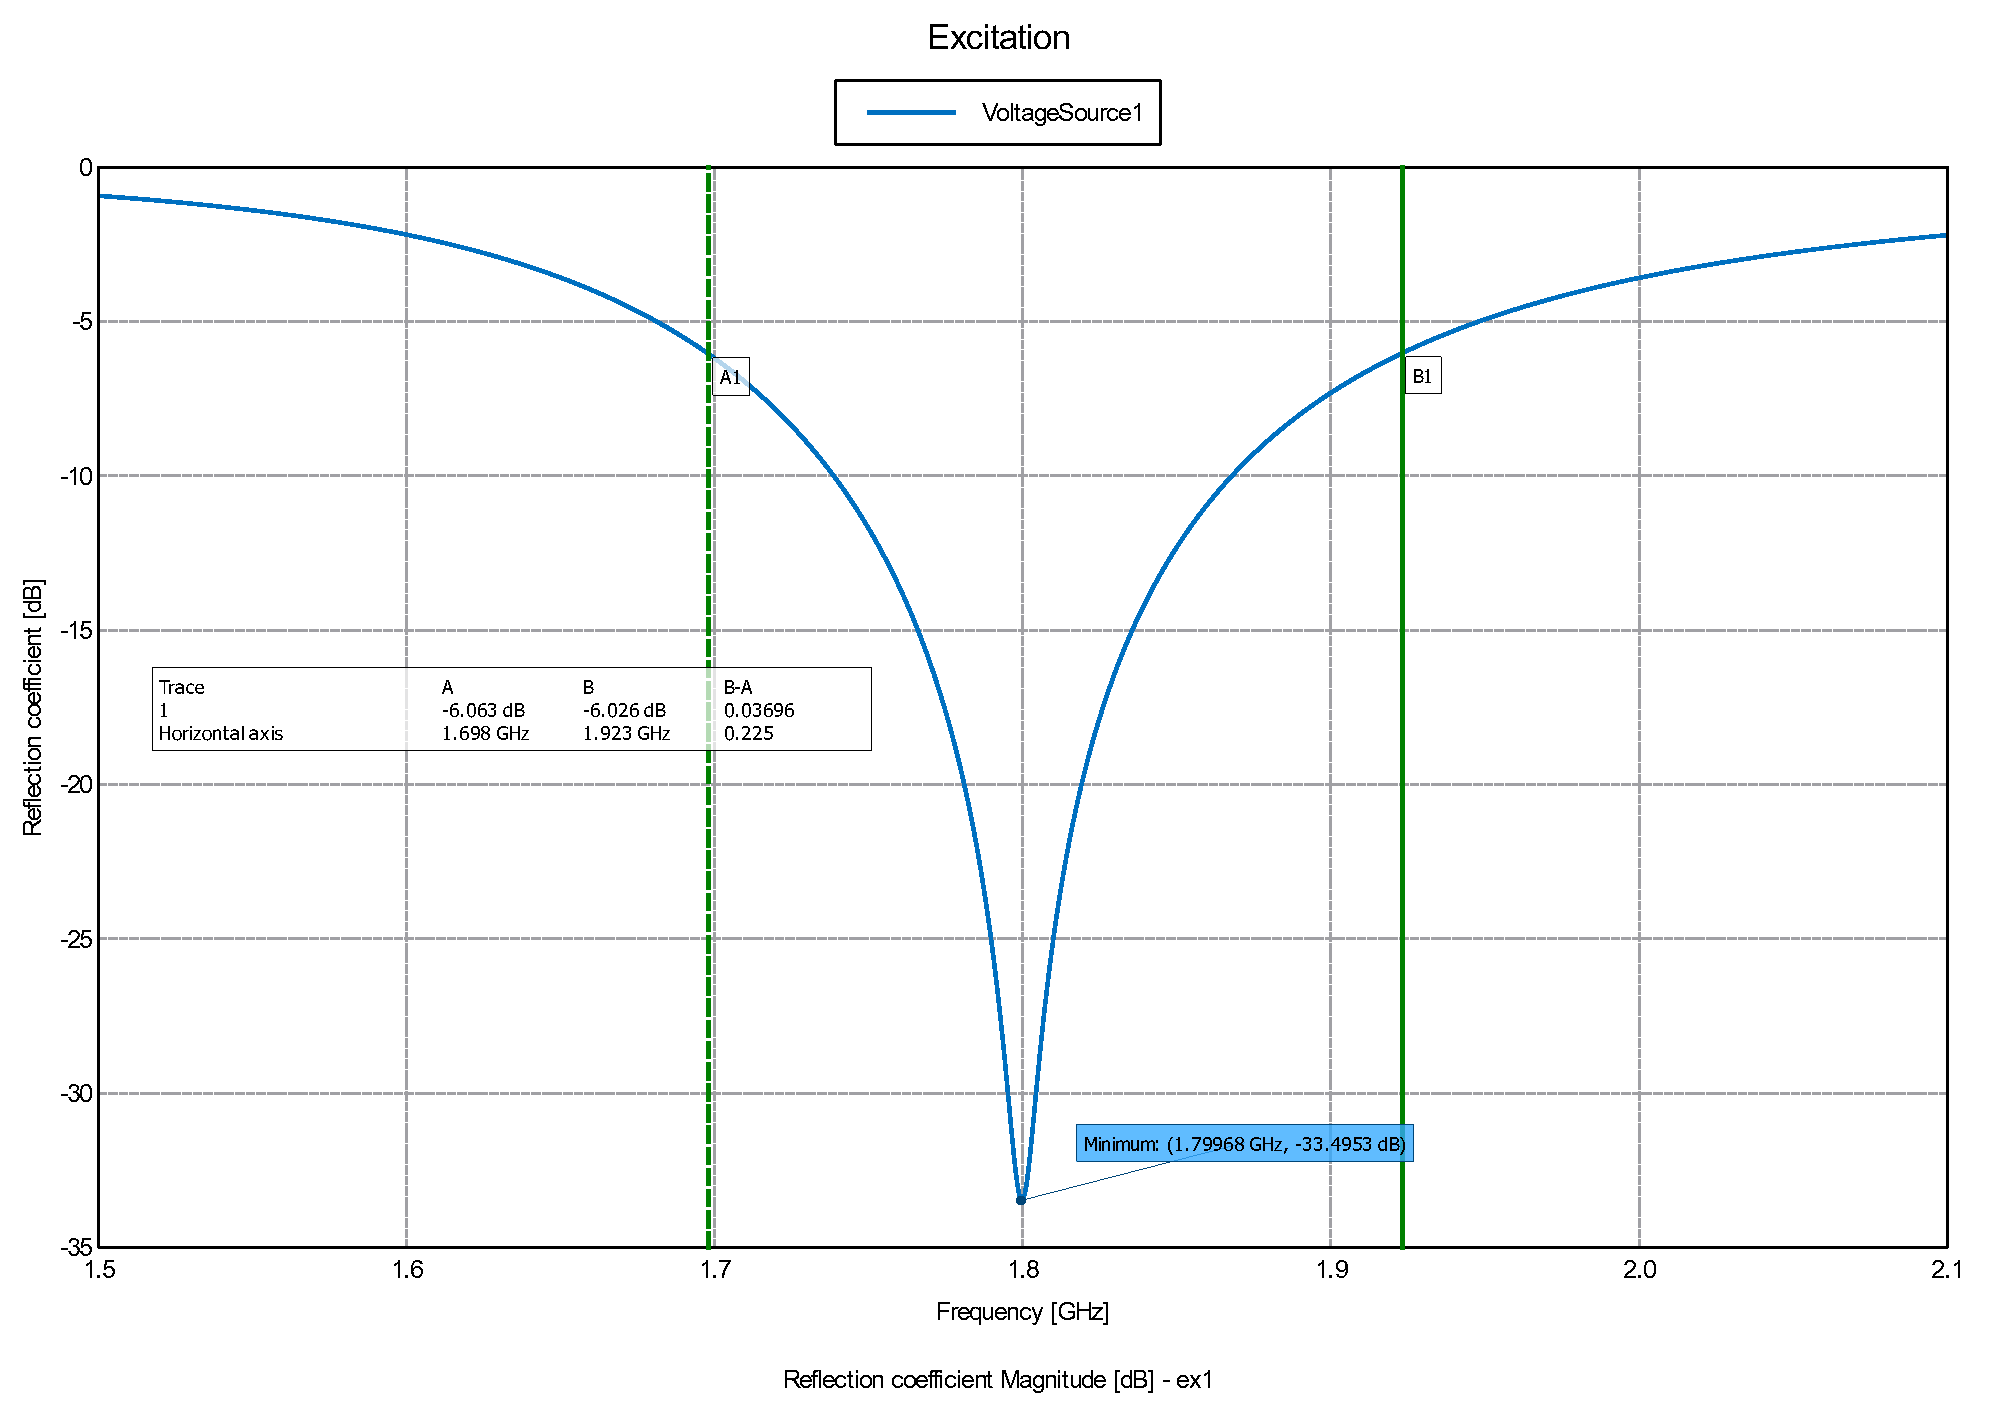
\includegraphics[width = \textwidth]{gamma22.pdf}
  \caption{$\Gamma_L$ de l'antenne dipôle adaptée pour \SI{1.8}{\giga\hertz} en fonction de la fréquence.\label{fig:gamma22}}
\end{figure}
De ce coefficient de réflexion on tire la fraction de puissance consommée à l'antenne par la relation \ref{eqn:puissance délivrée}.
\[
  \frac{P_L}{P_{in}} = \SI{99.9}{\percent}
\]

Jusqu'à présent, nous avons travaillé avec un diamètre de fil = $0.00001 \lambda$. Lorsqu'on multiplie ce diamètre par 50, on constate que la fréquence de résonance est légèrement diminuée, mais surtout que la bande passante est plus que doublée, comme le montre la figure \ref{fig:gamma5022}.
\begin{figure}[htbp]
  \centering
  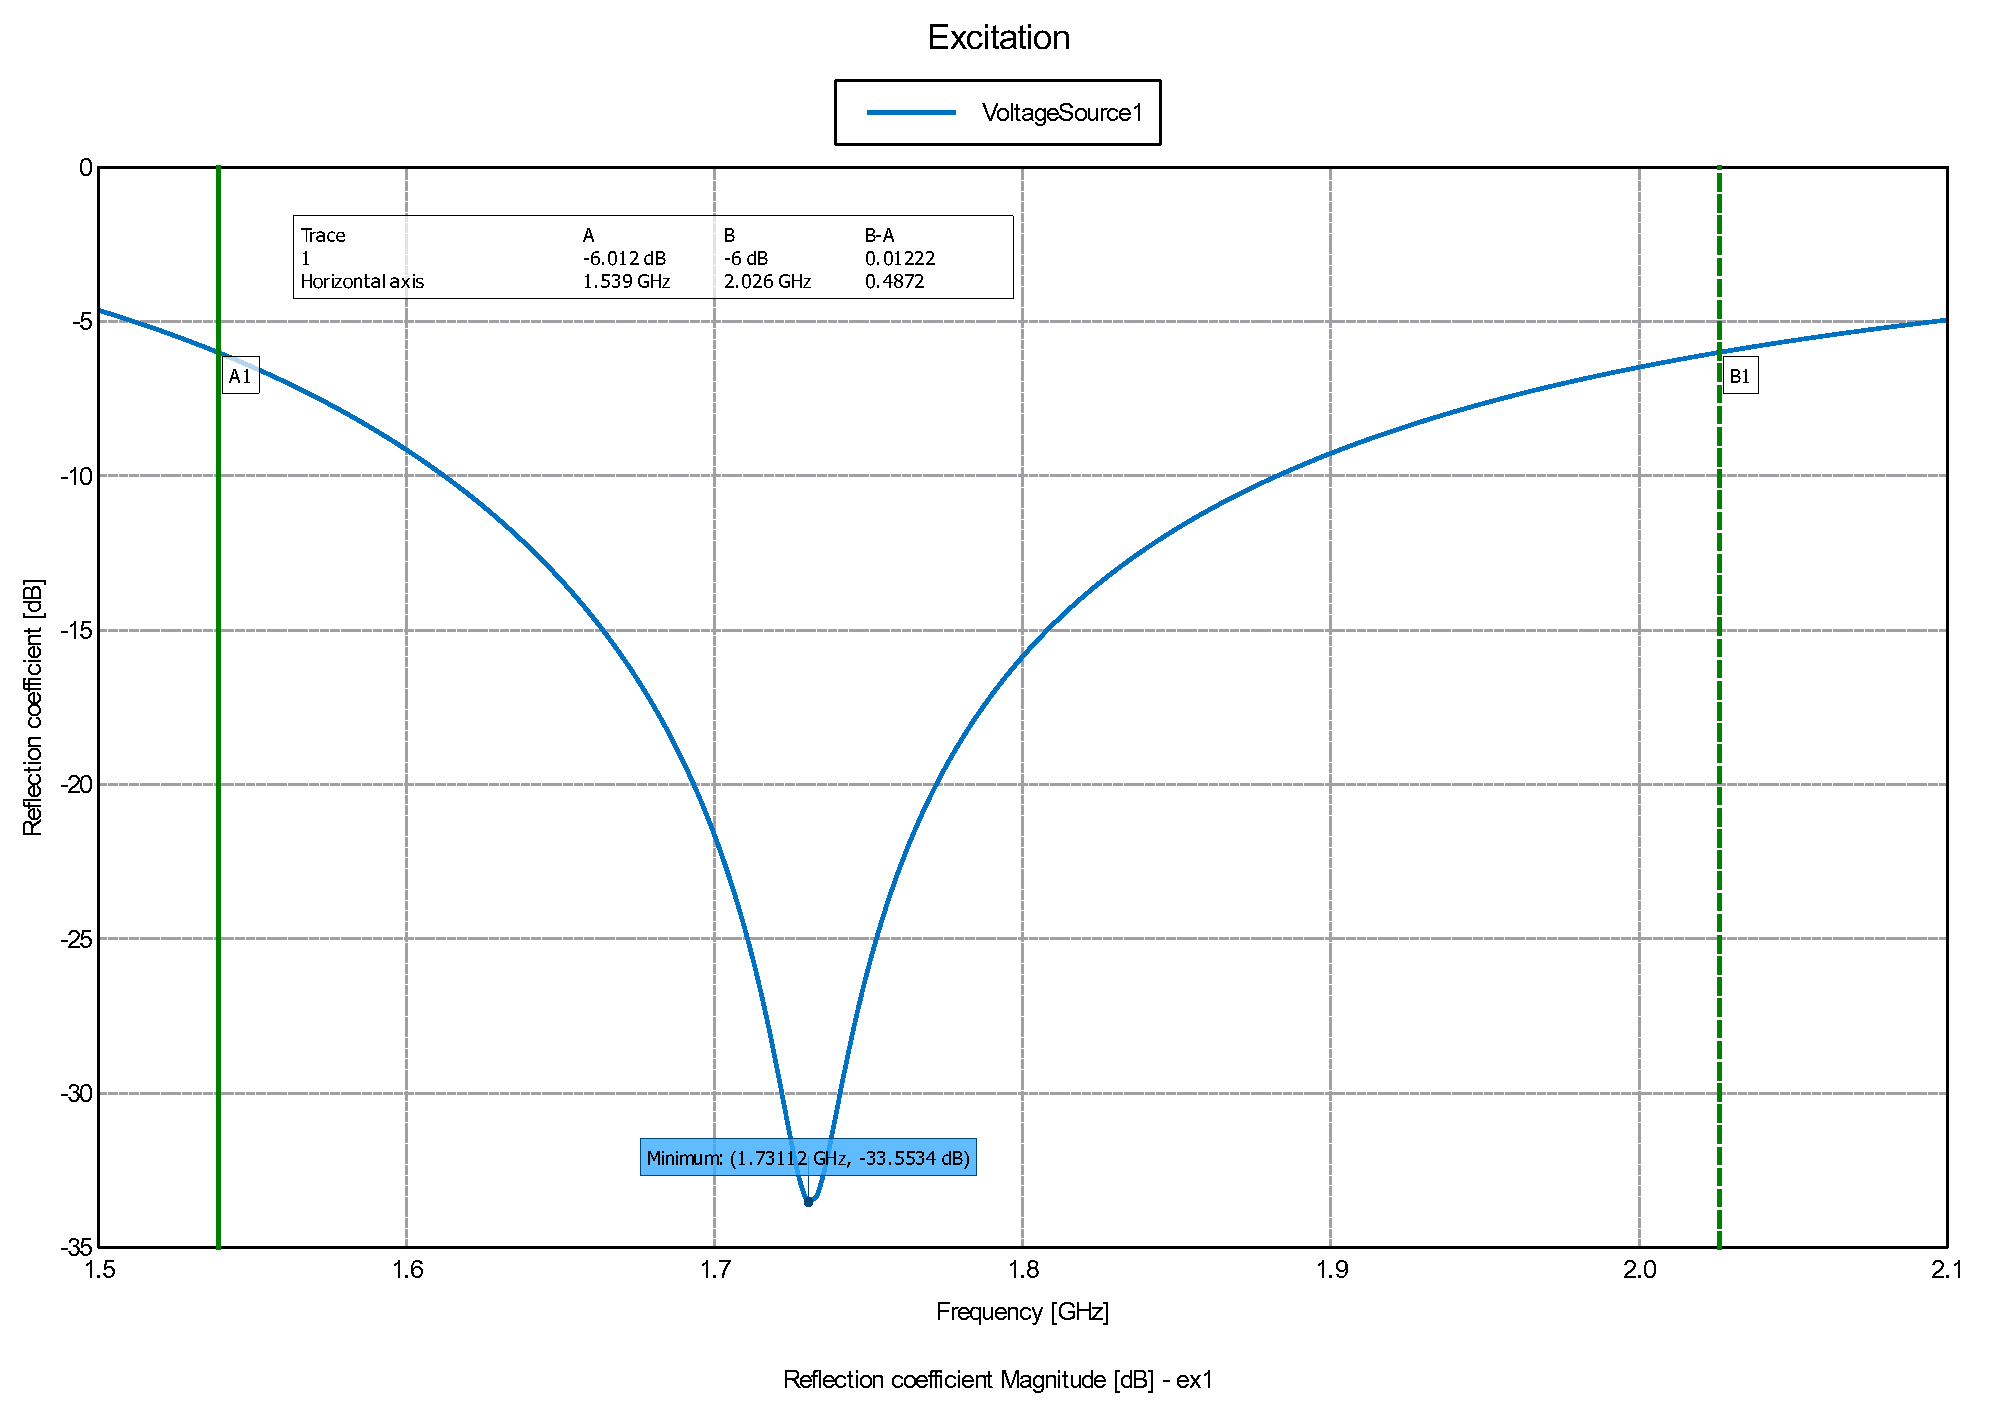
\includegraphics[width = \textwidth]{gamma5022.pdf}
  \caption{$\Gamma_L$  en fonction de la fréquence de l'antenne dipôle adaptée pour \SI{1.8}{\giga\hertz}, et diamètre multiplié par 50.\label{fig:gamma5022}}
\end{figure}
On constate en effet que la largeur de bande passe de \SI{225}{\mega\hertz} (figure \ref{fig:gamma22}) à \SI{487}{\mega\hertz} (figure \ref{fig:gamma5022}). Ceci s'explique par le fait qu'augmenter le diamètre du fil réduit la pente de $\Im(Z_L)$ en fonction de la fréquence.

\subsection{Le dipôle replié}





